% !TEX TS-program = pdflatex
% !TEX encoding = UTF-8 Unicode

% This is a simple template for a LaTeX document using the "article" class.
% See "book", "report", "letter" for other types of document.

\documentclass[10pt,twocolumn]{article}

\usepackage[utf8]{inputenc} % set input encoding (not needed with XeLaTeX)
\usepackage{graphicx}
\usepackage{listings} 
\usepackage{xcolor,colortbl}
\usepackage[section]{placeins}
\usepackage{amsthm}
\usepackage{mathtools}
\graphicspath{ {images/} }

%%% Examples of Article customizations
% These packages are optional, depending whether you want the features they provide.
% See the LaTeX Companion or other references for full information.

%%% PAGE DIMENSIONS
\usepackage{geometry} % to change the page dimensions
\geometry{a4paper} % or letterpaper (US) or a5paper or....
\geometry{margin=0.55in} % for example, change the margins to 2 inches all round
% \geometry{landscape} % set up the page for landscape
%   read geometry.pdf for detailed page layout information

\usepackage{graphicx} % support the \includegraphics command and options

% \usepackage[parfill]{parskip} % Activate to begin paragraphs with an empty line rather than an indent

%%% PACKAGES
\usepackage{booktabs} % for much better looking tables
\usepackage{array} % for better arrays (eg matrices) in maths
\usepackage{paralist} % very flexible & customisable lists (eg. enumerate/itemize, etc.)
\usepackage{verbatim} % adds environment for commenting out blocks of text & for better verbatim
\usepackage{subfig} % make it possible to include more than one captioned figure/table in a single float
\usepackage{indentfirst}
\usepackage{amsfonts}
\usepackage{amssymb}
\usepackage{amsthm}
\usepackage{tabularx}
% These packages are all incorporated in the memoir class to one degree or another...

%%% HEADERS & FOOTERS
\usepackage{fancyhdr} % This should be set AFTER setting up the page geometry
\pagestyle{fancy} % options: empty , plain , fancy
\renewcommand{\headrulewidth}{0pt} % customise the layout...
\lhead{}\chead{}\rhead{}
\lfoot{}\cfoot{\thepage}\rfoot{}

%%% SECTION TITLE APPEARANCE
\usepackage{sectsty}
\allsectionsfont{\sffamily\mdseries\upshape} % (See the fntguide.pdf for font help)
% (This matches ConTeXt defaults)

%%% ToC (table of contents) APPEARANCE
\usepackage[nottoc,notlof,notlot]{tocbibind} % Put the bibliography in the ToC
\usepackage[titles,subfigure]{tocloft} % Alter the style of the Table of Contents
\renewcommand{\cftsecfont}{\rmfamily\mdseries\upshape}
\renewcommand{\cftsecpagefont}{\rmfamily\mdseries\upshape} % No bold!
\setlength{\parindent}{0.5cm} 

%%% END Article customizations

%%% The "real" document content comes below...

\title{Redundant Primes In Goldbach Partitions}
\author{Marcin Barylski}
\date{\small{Published: October 13, 2019 \\ The last update: January 17, 2020}}

\definecolor{Gray}{gray}{0.85}
\definecolor{LightCyan}{rgb}{0.88,1,1}
\newcolumntype{a}{>{\columncolor{Gray}}c}
\newcolumntype{b}{>{\columncolor{white}}c}

\newtheorem{theorem}{Theorem}
\newtheorem{lemma}[theorem]{Lemma}

\newcommand\bigforall{\mbox{\huge $\mathsurround0pt\forall$}} 
\newcommand\bigexists{\mbox{\huge $\mathsurround0pt\exists$}} 

\begin{document}
\maketitle

\begin{abstract}
GoldbachStrong Conjecture ($GSC$), still unsolved, states that all even integers $n \textgreater 2$ can be expressed as the sum of two prime numbers (Goldbach partitions of $n$). But do we need all primes to satisfy this conjecture? This work is devoted to selection of must-have primes and formulation of stronger version of $GSC$ with reduced set of primes.
\end{abstract}

\section{Problem statement}

Goldbach Strong Conjecture ($GSC$, also called binary) asserts that all positive even integer $n$ $\geq$ 4 can be expressed as the sum of two prime numbers. This hypothesis, formulated by Goldbach in 1742 in letter to Euler \cite{goldbach1742} and then updated by Euler to the form above is one of the oldest and still unsolved problems in number theory. Empirical verification showed that it is true for all $n$ $\leq$ 4 x $10^{18}$ \cite{oliveira2012} \cite{oliveira2013}.\par
The expression of a given positive even number $n$ as a sum of two primes $p_1$ and $p_2$ is called a Goldbach Partition ($GP$) of $n$.  Let's denote this relation as $GSC(n, p_1, p_2)$. Then $GSC$ can be written as (1):

\begin{equation}
\displaystyle\mathop{\bigforall}_{x \textgreater 1, x \in \mathbb{N}} \displaystyle\mathop{\bigexists}_{p_1, p_2 \in \mathbb{P}} GSC (2x, p_1, p_2)
\end{equation}

But maybe we can formulate much stronger version of (1)? The set of prime numbers $\mathbb{P}$ is dense, number of $GP(n)$ is increasing with increasing $n$, thus question if stronger version $GSC$ is possible, raised in \cite{barylski2018}, is legitimate (2):

\begin{equation}
\displaystyle\mathop{\bigforall}_{x \textgreater 1, x \in \mathbb{N}} \displaystyle\mathop{\bigexists}_{p_1, p_2 \in \mathbb{R}} GSC (2x, p_1, p_2)
\end{equation}

where $\left\vert \mathbb{R} \right\vert \textless \left\vert \mathbb{P} \right\vert$. By design $\mathbb{R}$ contains primes only.

\section{Algorithm}

Elimination of primes must start from the fact that every prime is potentially required (Lemma 1).

\begin{lemma}
Every prime is present is some Goldbach partition of even number.
\end{lemma}
\begin{proof}
Let's assume that exists such prime $p$ that is not present in any Goldbach partition - we will show that this is not possible. $p + p$ is always even number, regardless $p$ is even or odd. This means that we have $GSC(2p, p, p)$ for any prime $p$ (in other words: $p$ is always in Goldbach partition of $2p$) what is in contrary to the initial assumption.
\end{proof}

Further elimination of primes from $\mathbb{P}$ to build $\mathbb{R}$ requires appropriate algorithm $A$ which is able to resign from a given prime, even if it is present in some $GPs$. Such algorithm $A$ could look as follows:

\begin{enumerate}
\item  Let $\mathbb{R}$ is empty, a set of $\mathbb{R}_i$ is empty and $n = 2$. Let's assume that we break calculations at $n = n_{max} \textgreater 2$.
\item  \textbf{New turn}: $n = n + 2$.
\item Break calculations if $n \textgreater n_{max}$.
\item  If  $\mathbb{R}$ is sufficient to fulfill GSC for all even numbers $q$ ($ 4 \leq q \leq n$), then go to \textbf{New turn}.
\item  If  we have a set of  $\mathbb{R}_i$ and any $\mathbb{R}_j$ belonging to this set is sufficient to fulfill GSC for all even numbers $q$ ($ 4 \leq q \leq n$), then $\mathbb{R} = \mathbb{R}_j$, we forget all $\mathbb{R}_i$ and go to \textbf{New turn}.
\item  If  not, find all $GP(n)$ and build as many candidates for $\mathbb{R}$ (let's call them $\mathbb{R}_i$) as required. As a base use either (as  a first choice) $\mathbb{R}$ (if $\mathbb{R}_i$ does not exist) or all previous $\mathbb{R}_i$ (if they are present).
\item Go to \textbf{New turn}.
\end{enumerate}

\section{Results}

Table 1 presents the very first rounds of algorithm eliminating primes required to satisfy $GSC$ - it is depicting current values of both $\mathbb{R}$ and $\mathbb{R}_i$, plus additional set $\mathbb{E}$ which contains primes that were present in $GPs$ so far but can be eliminated without hurting $GSC$. 

\begin{table}[ht]
\centering
\captionsetup{justification=centering}
\caption{Results of the first rounds of $A$}
\label{tablealgostart}
\begin{tabular}{lalalalal}
  \rowcolor{LightCyan}
  $n$ & $GP(n)$ & $\mathbb{R}$ & $\mathbb{R}_i$ & $\mathbb{E}$ \\
  \hline
4  & 2+2  & \{2\} & $\emptyset$ & $\emptyset$\\ 
  \hline
6  & 3+3 & \{2,3\} & $\emptyset$ & $\emptyset$\\ 
  \hline
8  & 3+5 & \{2,3,5\} & $\emptyset$ & $\emptyset$ \\
  \hline
10  & \begin{tabular}[c]{@{}l@{}}3+7\\5+5\end{tabular} & \{2,3,5\} & $\emptyset$ & \{7\} \\
  \hline
12  & 5+7 & \{2,3,5,7\} & $\emptyset$ & $\emptyset$ \\
  \hline
14  & \begin{tabular}[c]{@{}l@{}}3+11\\7+7\end{tabular} & \{2,3,5,7\} & $\emptyset$ & \{11\} \\
  \hline
16 & \begin{tabular}[c]{@{}l@{}}5+11\\3+13\end{tabular} &  $\emptyset$ & \begin{tabular}[c]{@{}l@{}}\{2,3,5,7,11\}\\\{2,3,5,7,13\}\end{tabular} & $\emptyset$ \\ 
  \hline
18 & \begin{tabular}[c]{@{}l@{}}5+13\\7+11\end{tabular} &  $\emptyset$ & \begin{tabular}[c]{@{}l@{}}\{2,3,5,7,11\}\\\{2,3,5,7,13\}\end{tabular} & $\emptyset$ \\ 
  \hline
20 & \begin{tabular}[c]{@{}l@{}}3+17\\7+13\end{tabular} & \{2,3,5,7,13\} & $\emptyset$ & \{11,17\} \\
  \hline                                                    
\end{tabular}
\end{table}

For instance, if we take into account all positive even numbers $2 \textless n \textless 16$, then we need a set of primes $\{2,3,5,7\}$ to satisfy $GSC$ for all $n$ checked so far and $\{11\}$ ($GSC(14, 3, 11)$) is our candidate for elimination.	

\begin{figure}[!ht]
\centering
\captionsetup{justification=centering}
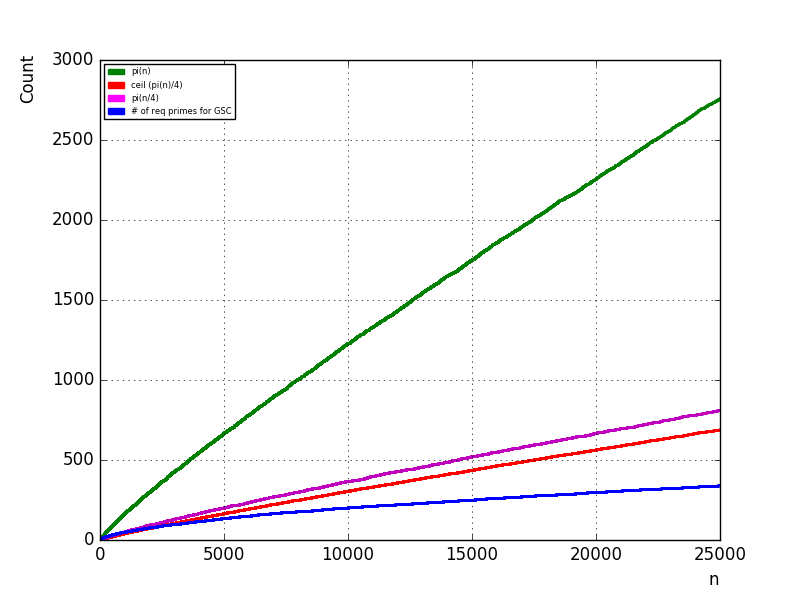
\includegraphics[width=9cm]{f_required_primes}
\caption[caption]{Required primes for GSC ($4 \leq n \leq 2.5 \times 10^4)$}
\label{fig:requiredprimes}
\end{figure}	

Figures 1, 2 and 3 are depicting findings after analyzing even numbers $4 \leq n \leq 2.5 \times 10^4$. First of all, function of required primes increases but slower than $\Pi(n)$.

\begin{figure}[!ht]
\centering
\captionsetup{justification=centering}
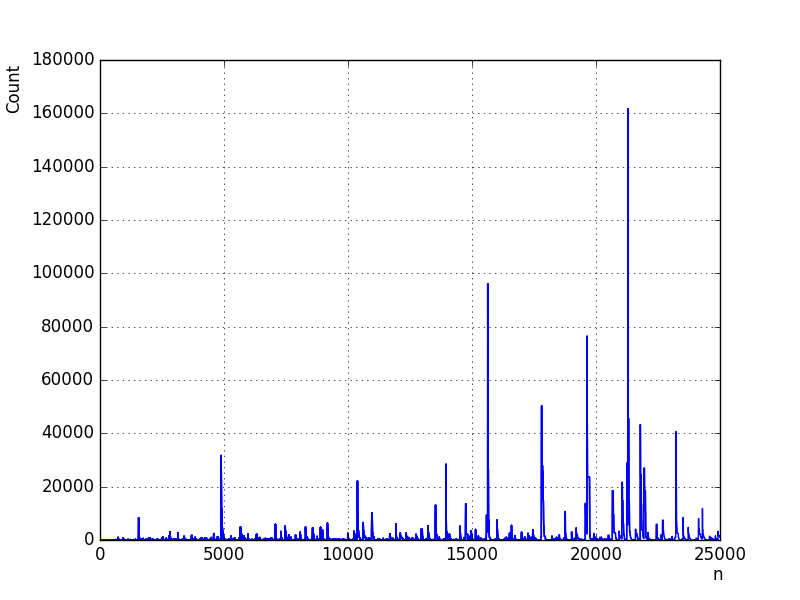
\includegraphics[width=9cm]{f_number_of_possible_sets}
\caption[caption]{Number of $\mathbb{R}_i$ ($4 \leq n \leq 2.5 \times 10^4$)}
\label{fig:numberofsets}
\end{figure}

It is also interesting that algorithm $A$ has sporadic congestions in terms of number of $\mathbb{R}_i$ - generally its number at a given time is low but there are quite frequent situation when it is high, even exceding 160000 (this means that we have 160000 subsets containing candidates for $\mathbb{R}$) - it happens when there are still some $\mathbb{R}_i$ and new $n$ requires new prime to be used which is multiplying number of $\mathbb{R}_i$ in next round. Surprisingly, shortly after number of $\mathbb{R}_i$ is decreasing to much smaller values. Congestions could be better handled (from memory utilization standpoint) if in $A$ instead of seperate lists (paths) we have a tree (where branches/leaves represent variable part added on top of common base).

\begin{figure}[!ht]
\centering
\captionsetup{justification=centering}
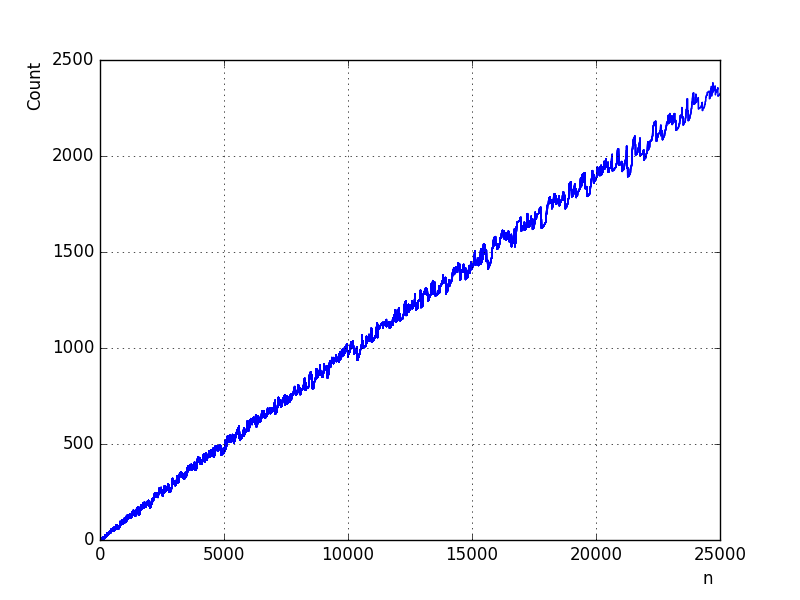
\includegraphics[width=9cm]{f_number_of_eliminated_primes}
\caption[caption]{Number of eliminated primes ($4 \leq n \leq 2.5 \times 10^4$)}
\label{fig:numberofeliminatedprimes}
\end{figure}

\begin{figure}[!ht]
\centering
\captionsetup{justification=centering}
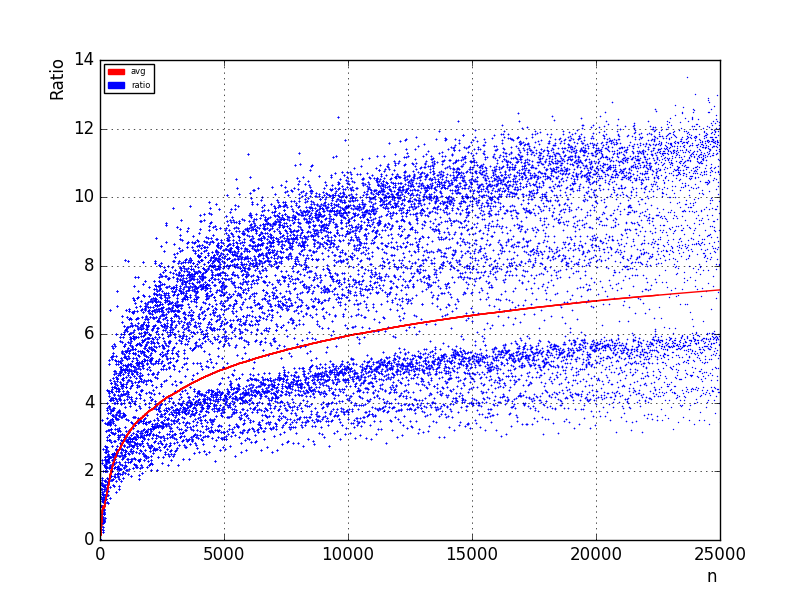
\includegraphics[width=9cm]{f_eliminated_primes_to_partitions}
\caption[caption]{Ratio of number of eliminated primes to number of GPs, including average value ($4 \leq n \leq 25 \times 10^3$)}
\label{fig:numberofeliminatedprimestopartitions}
\end{figure}

\section{Summary and next steps}

Executed experiments, run for all even $n \leq 2.5 \times 10^4$, confirmed that we do not need entire set of primes to satisfy $GSC$. Appendix A lists eliminated primes after checking all even $n \leq 2.5 \times 10^4$ - the smallest eliminated prime is $17$. Of course, exercised cases do not proof that eventually such set exists for all even $n$ but observed trends (Figure $\ref{fig:numberofeliminatedprimes}$, Figure $\ref{fig:numberofeliminatedprimestopartitions}$) give strong foundation that such set exists indeed and conjecture (2) is true. \par
As a result of this work one integer sequence has been submitted to OEIS database: A328179 \cite{A328179}. 

\begin{thebibliography}{9}
\bibitem{goldbach1742}
  Christian Goldbach, 
  \emph{On the margin of a letter to Leonard Euler},
  1742.
\bibitem{oliveira2012}
  Tomás Oliveira e Silva,
  \emph{Goldbach conjecture verification.}
  http://sweet.ua.pt/tos/goldbach.html,
  2012.
\bibitem{oliveira2013}
  Tomás Oliveira e Silva, Siegfried Herzog, and Silvio Pardi, 
  \emph{Empirical verification of the even Goldbach conjecture and computation of prime gaps up to 4 $\times 10^{18}$.}, 
  Mathematics of Computation, vol. 83, no. 288, pp. 2033-2060, 
  July 2014 (published electronically on November 18, 2013.
\bibitem{barylski2018}
  Marcin Barylski
  \emph{On $6k \pm 1$ Primes in Goldbach Strong Conjecture.}, 
  February 2018.
 \bibitem{A328179}
  OEIS Foundation Inc. (2019), The On-Line Encyclopedia of Integer Sequences, https://oeis.org/A328179. Number of distinct primes required to satisfy the Strong Goldbach Conjecture for all even numbers $\leq 2n$.

\appendix
\section{List of redundant primes}

Based on empirical verification done for all even numbers $4 \leq n \leq 25 \times 10^3$:

[17, 29, 43, 67, 71, 73, 83, 89, 103, 107, 131, 137, 157, 163, 167, 173, 179, 181, 193, 199, 229, 239, 241, 251, 257, 263, 269, 271, 277, 281, 283, 313, 317, 331, 349, 353, 359, 367, 401, 421, 431, 433, 443, 449, 463, 467, 479, 487, 499, 503, 509, 521, 523, 547, 557, 563, 571, 577, 587, 599, 601, 607, 617, 619, 631, 641, 643, 647, 659, 673, 677, 683, 691, 709, 719, 727, 733, 739, 751, 757, 761, 769, 773, 787, 797, 809, 811, 827, 829, 839, 853, 857, 859, 863, 883, 907, 911, 919, 937, 941, 947, 953, 967, 971, 977, 997, 1009, 1013, 1019, 1031, 1039, 1049, 1061, 1087, 1093, 1097, 1103, 1109, 1123, 1129, 1151, 1153, 1163, 1171, 1181, 1187, 1201, 1223, 1229, 1231, 1249, 1259, 1277, 1279, 1283, 1289, 1297, 1301, 1307, 1361, 1367, 1373, 1381, 1399, 1409, 1427, 1429, 1433, 1439, 1447, 1453, 1459, 1471, 1481, 1487, 1489, 1511, 1523, 1549, 1553, 1567, 1571, 1579, 1583, 1597, 1607, 1613, 1621, 1657, 1669, 1697, 1699, 1709, 1721, 1723, 1733, 1747, 1753, 1759, 1777, 1783, 1787, 1789, 1801, 1823, 1831, 1847, 1861, 1871, 1873, 1877, 1889, 1901, 1907, 1933, 1949, 1973, 1979, 1987, 1993, 1997, 2003, 2011, 2017, 2027, 2029, 2039, 2063, 2081, 2083, 2089, 2099, 2111, 2113, 2129, 2131, 2143, 2153, 2161, 2179, 2213, 2221, 2237, 2239, 2243, 2269, 2281, 2287, 2293, 2297, 2309, 2333, 2339, 2341, 2347, 2351, 2357, 2371, 2377, 2389, 2393, 2417, 2423, 2441, 2447, 2459, 2467, 2473, 2477, 2521, 2531, 2539, 2549, 2579, 2591, 2593, 2609, 2617, 2621, 2647, 2663, 2671, 2677, 2683, 2687, 2689, 2699, 2707, 2711, 2713, 2719, 2729, 2731, 2741, 2749, 2753, 2767, 2777, 2791, 2797, 2801, 2803, 2819, 2833, 2837, 2843, 2851, 2857, 2861, 2879, 2887, 2897, 2903, 2917, 2927, 2939, 2953, 2957, 2963, 2969, 2971, 2999, 3001, 3019, 3023, 3041, 3049, 3061, 3083, 3089, 3109, 3119, 3121, 3137, 3163, 3167, 3187, 3209, 3217, 3221, 3229, 3253, 3257, 3259, 3271, 3299, 3301, 3307, 3313, 3319, 3323, 3329, 3331, 3343, 3347, 3361, 3371, 3391, 3433, 3449, 3457, 3461, 3463, 3467, 3511, 3517, 3527, 3529, 3533, 3539, 3541, 3547, 3557, 3559, 3571, 3581, 3583, 3613, 3631, 3637, 3643, 3659, 3671, 3677, 3691, 3697, 3701, 3709, 3719, 3727, 3733, 3739, 3761, 3769, 3779, 3793, 3803, 3821, 3823, 3833, 3847, 3851, 3853, 3863, 3877, 3881, 3889, 3907, 3917, 3919, 3923, 3929, 3931, 3943, 3967, 3989, 4001, 4003, 4007, 4013, 4019, 4027, 4049, 4051, 4057, 4073, 4079, 4091, 4093, 4099, 4111, 4127, 4129, 4133, 4139, 4153, 4157, 4159, 4177, 4201, 4211, 4219, 4229, 4231, 4241, 4243, 4253, 4261, 4271, 4273, 4283, 4289, 4297, 4327, 4337, 4339, 4349, 4373, 4397, 4409, 4423, 4447, 4451, 4457, 4463, 4481, 4483, 4507, 4513, 4517, 4519, 4523, 4549, 4561, 4567, 4583, 4603, 4621, 4637, 4639, 4643, 4649, 4651, 4657, 4673, 4679, 4691, 4703, 4721, 4723, 4729, 4733, 4751, 4783, 4787, 4789, 4793, 4799, 4801, 4813, 4817, 4861, 4877, 4889, 4903, 4909, 4919, 4931, 4933, 4943, 4951, 4957, 4967, 4969, 4973, 4987, 4993, 4999, 5003, 5009, 5011, 5021, 5023, 5039, 5059, 5077, 5081, 5087, 5099, 5101, 5107, 5119, 5147, 5167, 5197, 5209, 5227, 5231, 5233, 5237, 5261, 5273, 5279, 5281, 5297, 5303, 5309, 5323, 5333, 5347, 5351, 5381, 5387, 5393, 5399, 5407, 5413, 5417, 5419, 5431, 5437, 5441, 5449, 5471, 5479, 5483, 5501, 5503, 5519, 5521, 5527, 5531, 5557, 5563, 5569, 5573, 5581, 5591, 5623, 5639, 5641, 5647, 5651, 5659, 5683, 5689, 5693, 5711, 5717, 5737, 5741, 5743, 5749, 5779, 5783, 5791, 5801, 5807, 5813, 5821, 5827, 5839, 5843, 5849, 5851, 5857, 5861, 5867, 5879, 5881, 5897, 5939, 5981, 5987, 6007, 6011, 6029, 6037, 6043, 6047, 6067, 6073, 6079, 6101, 6121, 6133, 6151, 6163, 6197, 6199, 6203, 6211, 6217, 6221, 6229, 6247, 6257, 6263, 6269, 6277, 6287, 6299, 6301, 6311, 6317, 6323, 6329, 6337, 6343, 6353, 6359, 6361, 6367, 6373, 6379, 6389, 6421, 6427, 6449, 6451, 6473, 6481, 6491, 6521, 6529, 6547, 6553, 6563, 6569, 6577, 6581, 6599, 6607, 6619, 6653, 6661, 6679, 6689, 6691, 6701, 6703, 6719, 6733, 6737, 6761, 6763, 6779, 6781, 6791, 6793, 6803, 6823, 6829, 6833, 6841, 6857, 6863, 6869, 6871, 6883, 6899, 6907, 6911, 6917, 6947, 6949, 6959, 6961, 6967, 6971, 6977, 6983, 6991, 6997, 7001, 7013, 7019, 7027, 7039, 7057, 7069, 7079, 7103, 7109, 7121, 7127, 7129, 7151, 7159, 7187, 7207, 7211, 7213, 7219, 7229, 7237, 7243, 7247, 7253, 7283, 7297, 7307, 7309, 7321, 7331, 7349, 7351, 7369, 7393, 7411, 7417, 7433, 7451, 7457, 7477, 7481, 7487, 7489, 7499, 7507, 7517, 7523, 7537, 7541, 7547, 7549, 7559, 7561, 7573, 7577, 7583, 7589, 7603, 7607, 7621, 7639, 7649, 7669, 7673, 7681, 7687, 7691, 7699, 7703, 7717, 7723, 7727, 7741, 7753, 7757, 7789, 7793, 7817, 7823, 7829, 7841, 7853, 7867, 7873, 7877, 7879, 7901, 7919, 7927, 7937, 7949, 7951, 7963, 8009, 8011, 8017, 8039, 8053, 8069, 8081, 8087, 8089, 8093, 8101, 8111, 8117, 8147, 8161, 8167, 8171, 8179, 8219, 8221, 8233, 8237, 8243, 8263, 8269, 8273, 8287, 8293, 8297, 8317, 8329, 8353, 8363, 8369, 8377, 8387, 8389, 8419, 8423, 8429, 8431, 8443, 8447, 8461, 8467, 8501, 8513, 8521, 8527, 8537, 8539, 8543, 8563, 8573, 8581, 8597, 8599, 8609, 8623, 8627, 8641, 8663, 8669, 8677, 8681, 8689, 8699, 8707, 8713, 8731, 8741, 8747, 8753, 8761, 8779, 8783, 8803, 8807, 8819, 8821, 8837, 8849, 8861, 8863, 8867, 8923, 8929, 8933, 8941, 8951, 8963, 8999, 9001, 9007, 9011, 9013, 9029, 9041, 9043, 9059, 9067, 9091, 9103, 9127, 9133, 9137, 9157, 9161, 9173, 9181, 9187, 9199, 9203, 9209, 9221, 9227, 9241, 9257, 9281, 9283, 9293, 9311, 9319, 9323, 9337, 9341, 9343, 9349, 9377, 9391, 9397, 9403, 9413, 9419, 9421, 9431, 9433, 9437, 9439, 9461, 9467, 9473, 9479, 9491, 9497, 9511, 9521, 9539, 9547, 9551, 9601, 9613, 9619, 9623, 9629, 9631, 9643, 9649, 9661, 9677, 9679, 9689, 9697, 9719, 9721, 9733, 9743, 9749, 9767, 9769, 9781, 9787, 9791, 9803, 9811, 9817, 9829, 9839, 9857, 9859, 9871, 9887, 9901, 9907, 9923, 9929, 9931, 9941, 9949, 9967, 9973, 10007, 10037, 10039, 10061, 10067, 10069, 10079, 10091, 10093, 10099, 10103, 10133, 10139, 10141, 10151, 10159, 10169, 10177, 10181, 10193, 10211, 10243, 10247, 10259, 10271, 10273, 10289, 10301, 10303, 10313, 10321, 10331, 10337, 10343, 10357, 10369, 10391, 10399, 10427, 10429, 10433, 10453, 10457, 10459, 10463, 10477, 10487, 10499, 10513, 10529, 10531, 10559, 10589, 10597, 10607, 10613, 10627, 10631, 10639, 10651, 10657, 10663, 10667, 10687, 10691, 10709, 10711, 10723, 10729, 10733, 10753, 10771, 10789, 10799, 10831, 10837, 10847, 10853, 10861, 10867, 10883, 10889, 10891, 10903, 10909, 10937, 10939, 10949, 10957, 10973, 10987, 10993, 11003, 11027, 11047, 11057, 11059, 11069, 11071, 11087, 11093, 11113, 11117, 11119, 11131, 11149, 11161, 11171, 11173, 11177, 11213, 11243, 11251, 11257, 11261, 11273, 11279, 11287, 11299, 11311, 11317, 11329, 11351, 11353, 11369, 11383, 11393, 11411, 11423, 11437, 11443, 11447, 11467, 11471, 11483, 11489, 11491, 11497, 11503, 11519, 11527, 11549, 11551, 11579, 11587, 11593, 11597, 11617, 11621, 11677, 11681, 11689, 11699, 11717, 11719, 11731, 11743, 11777, 11779, 11783, 11801, 11807, 11813, 11821, 11827, 11831, 11833, 11839, 11863, 11867, 11887, 11897, 11903, 11909, 11927, 11933, 11939, 11941, 11953, 11959, 11969, 11971, 11981, 11987, 12007, 12011, 12037, 12041, 12071, 12073, 12097, 12101, 12107, 12109, 12113, 12119, 12143, 12149, 12157, 12161, 12197, 12203, 12211, 12227, 12239, 12251, 12253, 12263, 12269, 12277, 12281, 12289, 12301, 12323, 12329, 12343, 12347, 12373, 12379, 12391, 12401, 12409, 12413, 12421, 12433, 12437, 12451, 12457, 12473, 12479, 12491, 12497, 12503, 12511, 12517, 12527, 12541, 12547, 12569, 12577, 12583, 12589, 12601, 12611, 12613, 12619, 12637, 12641, 12647, 12653, 12659, 12689, 12697, 12703, 12713, 12721, 12739, 12743, 12757, 12781, 12791, 12799, 12809, 12821, 12823, 12829, 12841, 12853, 12889, 12899, 12907, 12911, 12917, 12923, 12941, 12953, 12959, 12967, 12973, 12979, 12983, 13001, 13003, 13007, 13033, 13037, 13043, 13049, 13063, 13093, 13099, 13103, 13109, 13121, 13147, 13151, 13159, 13163, 13171, 13177, 13183, 13217, 13219, 13229, 13241, 13267, 13291, 13297, 13309, 13313, 13327, 13331, 13337, 13339, 13367, 13381, 13397, 13399, 13411, 13417, 13421, 13441, 13457, 13463, 13469, 13477, 13487, 13499, 13513, 13523, 13537, 13553, 13567, 13577, 13591, 13597, 13613, 13619, 13627, 13633, 13649, 13669, 13679, 13681, 13687, 13691, 13693, 13697, 13709, 13711, 13721, 13723, 13751, 13763, 13789, 13799, 13807, 13829, 13831, 13859, 13873, 13877, 13879, 13883, 13903, 13913, 13921, 13931, 13933, 13963, 13967, 13997, 13999, 14009, 14029, 14033, 14051, 14071, 14081, 14083, 14087, 14107, 14143, 14153, 14159, 14173, 14197, 14207, 14221, 14249, 14251, 14281, 14293, 14303, 14321, 14323, 14327, 14347, 14369, 14387, 14389, 14401, 14407, 14411, 14419, 14423, 14431, 14437, 14447, 14461, 14489, 14503, 14519, 14533, 14537, 14543, 14549, 14551, 14561, 14563, 14591, 14593, 14627, 14629, 14633, 14653, 14657, 14669, 14683, 14699, 14713, 14723, 14731, 14737, 14741, 14747, 14759, 14767, 14771, 14779, 14783, 14797, 14813, 14821, 14827, 14831, 14843, 14851, 14867, 14869, 14879, 14887, 14891, 14897, 14923, 14939, 14951, 14957, 14969, 14983, 15013, 15017, 15031, 15053, 15061, 15077, 15091, 15101, 15107, 15121, 15137, 15139, 15149, 15161, 15173, 15187, 15193, 15199, 15217, 15227, 15233, 15241, 15259, 15263, 15269, 15277, 15287, 15289, 15299, 15307, 15313, 15319, 15331, 15359, 15361, 15373, 15377, 15391, 15401, 15413, 15427, 15439, 15443, 15451, 15461, 15467, 15473, 15493, 15497, 15511, 15527, 15541, 15551, 15559, 15569, 15581, 15583, 15601, 15607, 15629, 15641, 15643, 15647, 15667, 15671, 15679, 15727, 15731, 15733, 15737, 15739, 15749, 15761, 15767, 15773, 15787, 15791, 15797, 15803, 15809, 15817, 15859, 15877, 15881, 15887, 15889, 15901, 15913, 15919, 15923, 15937, 15959, 15971, 15991, 16001, 16007, 16033, 16057, 16061, 16063, 16067, 16069, 16073, 16087, 16091, 16097, 16103, 16111, 16127, 16141, 16187, 16189, 16193, 16217, 16231, 16249, 16253, 16267, 16273, 16319, 16333, 16339, 16349, 16361, 16363, 16369, 16381, 16411, 16417, 16421, 16427, 16433, 16447, 16451, 16453, 16477, 16481, 16487, 16493, 16519, 16529, 16547, 16553, 16561, 16567, 16573, 16607, 16619, 16631, 16633, 16649, 16657, 16661, 16673, 16691, 16693, 16699, 16703, 16729, 16741, 16747, 16759, 16763, 16787, 16811, 16823, 16829, 16831, 16843, 16871, 16883, 16889, 16901, 16903, 16921, 16931, 16937, 16943, 16963, 16979, 16981, 16987, 16993, 17011, 17021, 17027, 17029, 17041, 17047, 17077, 17093, 17099, 17107, 17117, 17123, 17137, 17159, 17167, 17183, 17189, 17191, 17203, 17207, 17209, 17239, 17257, 17291, 17293, 17299, 17317, 17321, 17327, 17333, 17341, 17351, 17359, 17377, 17389, 17393, 17401, 17417, 17419, 17431, 17443, 17449, 17467, 17471, 17477, 17483, 17489, 17491, 17497, 17509, 17519, 17539, 17551, 17569, 17573, 17579, 17581, 17597, 17599, 17609, 17623, 17627, 17657, 17659, 17669, 17681, 17683, 17707, 17713, 17729, 17737, 17747, 17749, 17761, 17783, 17789, 17791, 17807, 17827, 17837, 17839, 17851, 17863, 17881, 17891, 17903, 17909, 17911, 17921, 17929, 17939, 17957, 17959, 17971, 17977, 17981, 17987, 17989, 18013, 18041, 18047, 18049, 18059, 18077, 18097, 18121, 18127, 18131, 18133, 18143, 18149, 18169, 18181, 18191, 18199, 18211, 18217, 18223, 18229, 18233, 18251, 18253, 18269, 18287, 18289, 18301, 18307, 18311, 18313, 18329, 18341, 18353, 18371, 18379, 18397, 18413, 18427, 18433, 18439, 18443, 18451, 18457, 18461, 18481, 18493, 18503, 18517, 18521, 18523, 18539, 18553, 18583, 18587, 18593, 18617, 18637, 18661, 18671, 18679, 18691, 18701, 18713, 18719, 18731, 18749, 18757, 18787, 18797, 18839, 18869, 18899, 18911, 18913, 18917, 18919, 18947, 18959, 18973, 18979, 19001, 19009, 19031, 19037, 19051, 19069, 19073, 19079, 19081, 19087, 19121, 19139, 19141, 19157, 19163, 19181, 19183, 19207, 19211, 19213, 19219, 19231, 19237, 19249, 19267, 19273, 19301, 19309, 19333, 19373, 19379, 19381, 19391, 19403, 19417, 19421, 19423, 19427, 19429, 19433, 19447, 19457, 19463, 19471, 19477, 19483, 19489, 19501, 19507, 19531, 19541, 19543, 19553, 19559, 19571, 19577, 19583, 19597, 19603, 19661, 19687, 19697, 19709, 19739, 19751, 19753, 19759, 19777, 19793, 19801, 19813, 19819, 19841, 19843, 19853, 19861, 19867, 19889, 19891, 19913, 19919, 19927, 19937, 19949, 19961, 19963, 19973, 19991, 19993, 19997, 20011, 20021, 20023, 20029, 20047, 20051, 20063, 20071, 20089, 20101, 20107, 20113, 20117, 20123, 20129, 20143, 20147, 20161, 20173, 20183, 20201, 20219, 20231, 20233, 20249, 20261, 20269, 20287, 20297, 20323, 20327, 20333, 20341, 20347, 20357, 20389, 20393, 20399, 20407, 20411, 20431, 20441, 20443, 20477, 20479, 20483, 20507, 20509, 20521, 20533, 20543, 20549, 20551, 20563, 20593, 20599, 20611, 20627, 20639, 20663, 20681, 20693, 20707, 20717, 20719, 20731, 20743, 20747, 20749, 20753, 20759, 20771, 20773, 20789, 20807, 20809, 20849, 20857, 20873, 20879, 20887, 20897, 20899, 20903, 20929, 20939, 20947, 20959, 20963, 20981, 20983, 21001, 21011, 21013, 21017, 21019, 21023, 21031, 21061, 21067, 21089, 21101, 21107, 21121, 21139, 21143, 21157, 21163, 21169, 21179, 21187, 21191, 21193, 21211, 21221, 21269, 21277, 21283, 21317, 21319, 21341, 21347, 21377, 21379, 21383, 21391, 21401, 21407, 21419, 21433, 21467, 21481, 21491, 21493, 21499, 21521, 21523, 21529, 21559, 21563, 21569, 21577, 21587, 21589, 21599, 21601, 21611, 21613, 21617, 21647, 21661, 21673, 21683, 21701, 21727, 21737, 21739, 21751, 21757, 21773, 21787, 21799, 21803, 21817, 21839, 21841, 21851, 21859, 21863, 21871, 21881, 21893, 21911, 21929, 21937, 21943, 21961, 21977, 21991, 21997, 22003, 22013, 22027, 22031, 22037, 22039, 22051, 22063, 22067, 22073, 22079, 22091, 22093, 22109, 22111, 22123, 22129, 22133, 22147, 22157, 22159, 22171, 22229, 22247, 22271, 22273, 22277, 22279, 22291, 22303, 22307, 22343, 22367, 22369, 22381, 22391, 22397, 22409, 22433, 22441, 22447, 22469, 22481, 22483, 22511, 22531, 22541, 22543, 22549, 22567, 22571, 22573, 22613, 22619, 22621, 22637, 22639, 22651, 22669, 22679, 22691, 22697, 22699, 22717, 22721, 22727, 22739, 22741, 22751, 22769, 22777, 22783, 22787, 22807, 22811, 22817, 22853, 22859, 22871, 22877, 22901, 22907, 22921, 22937, 22943, 22961, 22963, 22973, 22993, 23011, 23017, 23021, 23027, 23029, 23039, 23041, 23053, 23057, 23059, 23063, 23081, 23087, 23099, 23117, 23131, 23143, 23159, 23167, 23189, 23197, 23201, 23209, 23227, 23251, 23291, 23293, 23311, 23321, 23327, 23333, 23339, 23369, 23371, 23399, 23431, 23447, 23459, 23473, 23497, 23531, 23537, 23539, 23549, 23557, 23561, 23563, 23567, 23581, 23593, 23603, 23609, 23623, 23627, 23629, 23633, 23663, 23669, 23671, 23677, 23687, 23689, 23719, 23741, 23747, 23753, 23767, 23773, 23789, 23801, 23813, 23819, 23827, 23833, 23857, 23869, 23873, 23879, 23887, 23893, 23899, 23909, 23911, 23917, 23929, 23957, 23971, 23977, 23981, 23993, 24001, 24007, 24019, 24023, 24043, 24049, 24061, 24071, 24077, 24083, 24091, 24097, 24103, 24107, 24109, 24113, 24121, 24133, 24137, 24169, 24179, 24181, 24197, 24203, 24223, 24229, 24239, 24247, 24251, 24281, 24317, 24329, 24359, 24371, 24391, 24407, 24413, 24419, 24421, 24443, 24469, 24473, 24481, 24499, 24509, 24517, 24547, 24551, 24571, 24611, 24631, 24659, 24671, 24677, 24691, 24697, 24749, 24763, 24821, 24841, 24847, 24851, 24859, 24877, 24889, 24907, 24917, 24919, 24923, 24943, 24953, 24967, 24971, 24977, 24979, 24989]

\end{thebibliography}

\end{document}
